\documentclass[journal,12pt,twocolumn]{IEEEtran}

\usepackage{setspace}
\usepackage{gensymb}
\singlespacing
\usepackage[cmex10]{amsmath}

\usepackage{amsthm}

\usepackage{mathrsfs}
\usepackage{txfonts}
\usepackage{stfloats}
\usepackage{bm}
\usepackage{cite}
\usepackage{cases}
\usepackage{subfig}

\usepackage{longtable}
\usepackage{multirow}

\usepackage{enumitem}
\usepackage{mathtools}
\usepackage{steinmetz}
\usepackage{tikz}
\usepackage{circuitikz}
\usepackage{verbatim}
\usepackage{tfrupee}
\usepackage[breaklinks=true]{hyperref}
\usepackage{graphicx}
\usepackage{tkz-euclide}

\usetikzlibrary{calc,math}
\usepackage{listings}
    \usepackage{color}                                            %%
    \usepackage{array}                                            %%
    \usepackage{longtable}                                        %%
    \usepackage{calc}                                             %%
    \usepackage{multirow}                                         %%
    \usepackage{hhline}                                           %%
    \usepackage{ifthen}                                           %%
    \usepackage{lscape}     
\usepackage{multicol}
\usepackage{chngcntr}
\usepackage{float}
\restylefloat{table}

\DeclareMathOperator*{\Res}{Res}

\renewcommand\thesection{\arabic{section}}
\renewcommand\thesubsection{\thesection.\arabic{subsection}}
\renewcommand\thesubsubsection{\thesubsection.\arabic{subsubsection}}

\renewcommand\thesectiondis{\arabic{section}}
\renewcommand\thesubsectiondis{\thesectiondis.\arabic{subsection}}
\renewcommand\thesubsubsectiondis{\thesubsectiondis.\arabic{subsubsection}}


\hyphenation{op-tical net-works semi-conduc-tor}
\def\inputGnumericTable{}                                 %%

\lstset{
%language=C,
frame=single, 
breaklines=true,
columns=fullflexible
}
\begin{document}

\newcommand{\BEQA}{\begin{eqnarray}}
\newcommand{\EEQA}{\end{eqnarray}}
\newcommand{\define}{\stackrel{\triangle}{=}}
\bibliographystyle{IEEEtran}
\raggedbottom
\setlength{\parindent}{0pt}
\providecommand{\mbf}{\mathbf}
\providecommand{\pr}[1]{\ensuremath{\Pr\left(#1\right)}}
\providecommand{\qfunc}[1]{\ensuremath{Q\left(#1\right)}}
\providecommand{\sbrak}[1]{\ensuremath{{}\left[#1\right]}}
\providecommand{\lsbrak}[1]{\ensuremath{{}\left[#1\right.}}
\providecommand{\rsbrak}[1]{\ensuremath{{}\left.#1\right]}}
\providecommand{\brak}[1]{\ensuremath{\left(#1\right)}}
\providecommand{\lbrak}[1]{\ensuremath{\left(#1\right.}}
\providecommand{\rbrak}[1]{\ensuremath{\left.#1\right)}}
\providecommand{\cbrak}[1]{\ensuremath{\left\{#1\right\}}}
\providecommand{\lcbrak}[1]{\ensuremath{\left\{#1\right.}}
\providecommand{\rcbrak}[1]{\ensuremath{\left.#1\right\}}}
\theoremstyle{remark}
\newtheorem{rem}{Remark}
\newcommand{\sgn}{\mathop{\mathrm{sgn}}}
\providecommand{\abs}[1]{\vert#1\vert}
\providecommand{\res}[1]{\Res\displaylimits_{#1}} 
\providecommand{\norm}[1]{\lVert#1\rVert}
%\providecommand{\norm}[1]{\lVert#1\rVert}
\providecommand{\mtx}[1]{\mathbf{#1}}
\providecommand{\mean}[1]{E[ #1 ]}
\providecommand{\fourier}{\overset{\mathcal{F}}{ \rightleftharpoons}}
%\providecommand{\hilbert}{\overset{\mathcal{H}}{ \rightleftharpoons}}
\providecommand{\system}{\overset{\mathcal{H}}{ \longleftrightarrow}}
	%\newcommand{\solution}[2]{\textbf{Solution:}{#1}}
\newcommand{\solution}{\noindent \textbf{Solution: }}
\newcommand{\cosec}{\,\text{cosec}\,}
\providecommand{\dec}[2]{\ensuremath{\overset{#1}{\underset{#2}{\gtrless}}}}
\newcommand{\myvec}[1]{\ensuremath{\begin{pmatrix}#1\end{pmatrix}}}
\newcommand{\mydet}[1]{\ensuremath{\begin{vmatrix}#1\end{vmatrix}}}
\numberwithin{equation}{subsection}
\makeatletter
\@addtoreset{figure}{problem}
\makeatother
\let\StandardTheFigure\thefigure
\let\vec\mathbf
\renewcommand{\thefigure}{\theproblem}
\def\putbox#1#2#3{\makebox[0in][l]{\makebox[#1][l]{}\raisebox{\baselineskip}[0in][0in]{\raisebox{#2}[0in][0in]{#3}}}}
     \def\rightbox#1{\makebox[0in][r]{#1}}
     \def\centbox#1{\makebox[0in]{#1}}
     \def\topbox#1{\raisebox{-\baselineskip}[0in][0in]{#1}}
     \def\midbox#1{\raisebox{-0.5\baselineskip}[0in][0in]{#1}}
\vspace{3cm}
\title{AI1103-Assignment 3}
\author{W Vaishnavi\\AI20BTECH11025}
\maketitle
\newpage
\bigskip
\renewcommand{\thefigure}{\theenumi}
\renewcommand{\thetable}{\theenumi}
Download all python codes from 
%
\begin{lstlisting}
https://github.com/vaishnavi-w/AI1103/blob/main/Assignment3/code3.py
\end{lstlisting}
and latex-tikz codes from 
%
\begin{lstlisting}
https://github.com/vaishnavi-w/AI1103/blob/main/Assignment3/latex3.tex
\end{lstlisting}
\section*{Question}
Probability density function $p(x)$ of random variable x is as shown below. The value of a is
\begin{enumerate}[label=\Alph*)]
    \item $\frac{2}{c}$
    \item $\frac{1}{c}$
    \item $\frac{2}{(b+c)}$
    \item $\frac{1}{(b+c)}$
\end{enumerate}
\begin{figure}[h!]
\centering
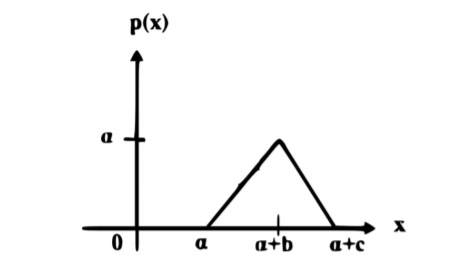
\includegraphics[width=\columnwidth]{convolution.png}
\caption{PDF}
\label{fig:BSC}
\end{figure}
\section*{Solution}

Let $Y_1$ and $Y_2$ be two independent and identically distributed (IID) random variables.\\
Let X be a random variable such that
\begin{align}
    X = Y_1 + Y_2
\end{align}
Let
\begin{align}
    p_{Y_1}\brak{y} &= \Pr\brak{Y_1=y} \\
    p_{Y_2}\brak{y} &= \Pr\brak{Y_2=y} \\
    p_X\brak{x} &= \Pr\brak{X=x}
\end{align}
be the probability densities of random variables $Y_1, Y_2$ and $X$. \\
$Y_1$ and $Y_2$ lie in the range ($\frac{a}{2}$,$\frac{a+c}{2}$), therefore,
\begin{align}
    \int_{\frac{a}{2}}^{\frac{a+c}{2}} p_{Y_1}\brak{y} \,dy  &=1 \\
    \frac{c}{2} \times p_{Y_1}\brak{y}  &= 1 \\
     p_{Y_1}\brak{y} &= \frac{2}{c}
\end{align}
The PDF for $Y_1$ and $Y_2$,
\begin{align}
p_{Y_1}(y) = p_{Y_2}(y) = 
\begin{cases}
\frac{2}{c} &  \frac{a}{2} \le y \le \frac{a+c}{2}\\
0 & \text{otherwise}
\end{cases}
\end{align}

The density of X is obtained by convolution of $Y_1$ and $Y_2$
\begin{align}
p_X(x) =  \int_{- \infty}^{\infty} p_{Y_1}(x-y)p_{Y_2}(y) \,dy
\end{align}
We have,
\begin{align}
    X = Y_1 + Y_2 \implies x = 2y\\
    \label{eq1} \frac{a}{2}\leq y \leq \frac{a+c}{2}\\ 
    \frac{a}{2}\le x-y \le \frac{a+c}{2}\\
    \label{eq2} x-\frac{a+c}{2}\le y \le x-\frac{a}{2}
\end{align}
From \eqref{eq1} and \eqref{eq2}
\begin{multline}
    \max\brak{\frac{a}{2}, x-\frac{a+c}{2}}\le y \le\\
    \min\brak{\frac{a+c}{2}, x-\frac{a}{2}}
\end{multline}
When $a \le x \le \frac{a+c}{2}$
\begin{align}
    p_X(x) & = \int_{\frac{a}{2}}^{x-\frac{a}{2}} p_{Y_1}(x-y)p_{Y_2}(y)\,dy\\
    & = \int_{\frac{a}{2}}^{x-\frac{a}{2}} \frac{2}{c}\times\frac{2}{c}\,dy\\
    & = \frac{4}{c^2}\brak{x-a}
\end{align}
Similarly, when $\frac{a+c}{2} \le x \le a+c $
\begin{align}
    p_X(x) & = \int_{x-\frac{a+c}{2}}^{\frac{a+c}{2}} p_{Y_1}(x-y)p_{Y_2}(y)\,dy\\
    & = \frac{4}{c^2}\brak{a+c-x}
\end{align}
The PDF of X is,
\begin{align}
p_x = 
\begin{cases}
\frac{4}{c^2}\brak{x-a} & a \le x \le a+\frac{c}{2}\\
\frac{4}{c^2}\brak{a+c-x} & a+\frac{c}{2} \le x \le a+c \\
0 & \text{otherwise}
\end{cases}
\end{align}
\begin{figure}[h!]
\centering
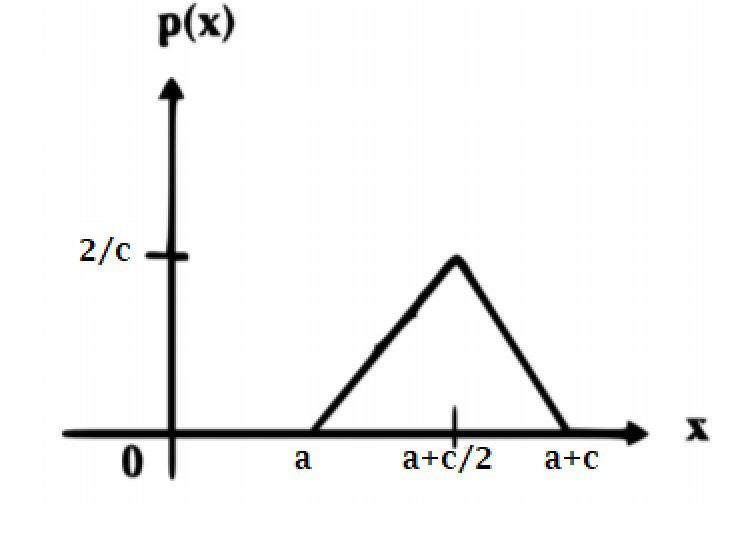
\includegraphics[width=\columnwidth]{conv.png}
\caption{PDF of X}
\label{fig:convolution}
\end{figure}
Thus, the PDF of X is,\\
The PDF of X from Figure.\ref{fig:BSC} in the question,
\begin{align}
p_x = 
\begin{cases}
\frac{a}{b}\brak{x-a} & a \le x \le a+b\\
\frac{a}{b-c}\brak{a+c-x} & a+b \le x \le a+c \\
0 & \text{otherwise}
\end{cases}
\end{align}

On comparing the parameters, we have
\begin{align}
    b=\frac{c}{2}\\
    a=\frac{2}{c}
\end{align}
\rightline{Answer : Option A}
\section*{Verification}
Verifying the result obtained with numerical values:\\
Let $a=1$.\\
\because a=\frac{2}{c} \implies c=2\\

The PDF of X is,
\begin{align}
p_x = 
\begin{cases}
\brak{x-1} & 1 \le x \le 2\\
\brak{3-x} & 2 \le x \le 3 \\
0 & \text{otherwise}
\end{cases}
\end{align}
CDF of X is defined as,
\begin{align}
    F_X\brak{x}=\pr{X \le x}
\end{align}
For $x \le 2$,
\begin{align}
    \pr{X \le x}& = \int_{- \infty}^{x} p_X\brak{x} \,dx\\
    & = \int_{1}^{x} x-1 \,dx\\
    & = \frac{x^2-2x+1}{2}
\end{align}

For $x \le 3$,
\begin{align}
    \pr{X \le x}& = \int_{- \infty}^{x} p_X\brak{x} \,dx\\
    & = \frac{1}{2} + \int_{2}^{x} 3-x \,dx\\
    & = \frac{6x-x^2-7}{2}
\end{align}
The CDF of X,
\begin{align}
F_X\brak{x} = 
\begin{cases}
0 & x < 1\\
\frac{x^2-2x+1}{2} &  x \le 2\\
\frac{6x-x^2-7}{2} & x \le 3 \\
1 & x > 3
\end{cases}
\end{align}
The plots for CDF and PDF of $X$ are given in Figure \ref{fig:cdf3} and Figure \ref{fig:pdf3}
\begin{figure}[h!]
\centering
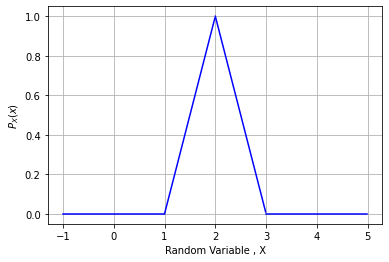
\includegraphics[width=\columnwidth]{pdf3.png}
\caption{PDF of X}
\label{fig:pdf3}
\end{figure}
\begin{figure}[h!]
\centering
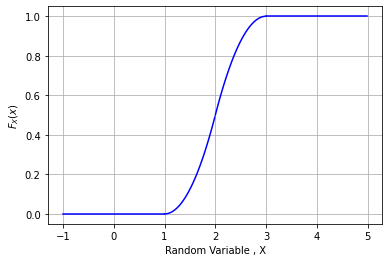
\includegraphics[width=\columnwidth]{cdf3.png}
\caption{CDF of X}
\label{fig:cdf3}
\end{figure}
\end{document}
